\documentclass[16pts]{report}
\usepackage[utf8]{inputenc}
\usepackage[T1]{fontenc}
\usepackage[francais]{babel}
\usepackage{xcolor}
\usepackage[hyphens]{url}
\usepackage[hidelinks]{hyperref}
\usepackage{amsmath}
\usepackage{graphicx}
\usepackage{geometry}
\usepackage{textcomp}
\hypersetup{hypertexnames=true}
\geometry{hmargin=2.5cm,vmargin=1.5cm}

%\maketitle
%\clearpage

\begin{document}
\bibliographystyle{unsrt}
\nocite{*}

\chapter{Besoins fonctionnels}
\label{cha:Besoins fonctionnels}


\section{Mots-clés et description d'une option}
\label{sec:Mots-clés et description d'une option}

Un utilisateur doit pouvoir sélectionner une option et y ajouter un mot-clé.
Par exemple, il peut spécifier qu'une option possède le mot-clé "Network". Il
pourra également supprimer et modifier les mots-clés existants. De la même
façon, l'utilisateur pourra éditer la description d'une option.

\section{Recherche}
\label{sec:Recherche}

L'utilisateur doit pouvoir effectuer une recherche sur le nom, la description
et les mots-clés d'une option lors de la configuration du noyau. La fonction de
recherche ne posera pas de véritable problème technique. L'utilisateur pourra
faire défiler les lignes contenant les occurences du terme recherché.

\section{Détection du matériel}
\label{sec:Détection du matériel}

La génération d'une configuration prédéfinie par détection du matériel hôte est
un besoin fonctionnel. En effet, un utilisateur ne voulant que le minimum
nécessaire dans son noyau est confronté à ce souci de recherche et de
correspondance de module au matériel.
Il existe des outils Linux permettant de récupérer la liste du matériel associé
aux bus PCI et USB de la machine hôte.
N'ayant pas trouvé d'outils Linux permettant de récupérer directement le ou les
modules noyau utilisés sur une entrée, l'étude du contenu des répertoires "/dev
/sys" et "/proc" sera nécessaire afin d'acquérir de plus amples informations.
Afin de rendre la correspondance des modules du noyau Linux au matériel plus
pertinente et fiable, l'idée serait de récupérer des logs d'exécution du scan
du matériel afin de peupler de manière volontaire une base de donnée
communautaire.

\section{Génération du fichier .config}
\label{sec:Génération du fichier .config}

L'utilisateur doit pouvoir sauvegarder où il le souhaite le fichier de
configuration généré par l'application. Un message (sous la forme d'une pop-up)
avertira l'utilisateur de la présence de conflits ou d'erreurs de dépendance
avant que la génération ne soit faite.

\section{Gestion des conflits}
\label{sec:Gestion des conflits}

L'application doit pouvoir "gérer les conflits et les dépendances" entre les
options de configuration. Grâce au fichier kconfig, l'application pourra, pour
chaque option de configuration, connaître ses dépendances et les options avec
lesquelles elle rentre en conflit. De ce fait chaque fois que l'utilisateur
sélectionne ou désélectionne une option de configuration, des tests sont
effectués pour savoir si cette option entre en conflit avec une autre (si elle
est cochée) ou génère une erreur de dépendance (si elle est décochée).

\section{Chargement d'un fichier .config}
\label{sec:Chargement d'un fichier .config}

La reprise d'un fichier .config doit permettre à un utilisateur de charger une
configuration existante. Le chargement d'un fichier .config corrompu provoquera
une erreur, et les options inconnues (s'il y en a) seront simplement ignorées.
Cela impliquera le déclenchement du mécanisme de résolution des conflits.

\section{Plateforme de partage communautaire}
\label{sec:Plateforme de partage communautaire}

S'il le souhaite, l'utilisateur peut envoyer sur la plateforme de partage, la
correspondance entre le matériel et le module capable de le faire fonctionner,
enrichissant ainsi la base de données de la plateforme.
De la même façon, lors de la détection du matériel, l'application pourra
trouver les modules à activer (dans le fichier .config) grâce à cette
plateforme. Celle-ci servira également à stocker les "descriptions" et les
mots-clés des options.


\chapter{Besoins non fonctionnnels}
\label{cha:Besoins non fonctionnnels}

\section{Facilité d'utilisation}
\label{sec:Facilité d'utilisation}

Notre projet consiste à améliorer l'utilisation des fonctionnalités de base des
outils existants, en les rendant plus accessibles. On a pu constater que le
système de recherche des options n'est pas simple à prendre en main et que la
gestion des conflits pouvait être améliorée.
Nous avons décidé d'améliorer la recherche en scrutant au sein des descriptions
des options en plus de leurs noms. De plus, nous affichons les options pouvant
créer des conflits, ainsi que des informations sur leur provenance.


\section{Profil utilisateur}
\label{sec:Profil utilisateur}

Actuellement, les outils de configuration d'un noyau Linux sont "réservés" aux
personnes averties. Il faut donc que les fonctionnalités recherchées soient
présentes. Ces améliorations permettront de toucher un plus large public, de
débutant à expert.


\section{Portabilité}
\label{sec:Portabilité}

Il y a deux aspects liés à la portabilité.
Dans un premier temps, il est possible que l'environnement dans lequel
l'application sera exécutée ne possède pas de serveur X (interface graphique).
Par conséquent, une solution privilégiant une interface console (comme Ncurse)
serait donc intéressante puisqu'elle conviendrait à la fois à l'utilisation de
l'application sur un serveur et sur un ordinateur personnel (ou même sur tout
type de support supportant un noyau Linux). Cependant, l'application se voulant
être tout public, une interface lancée depuis la console pourrait se montrer un
peu austère pour un utilisateur habitué à une interface graphique plus
"traditionnelle".

Dans un second temps, l'application pourra être fonctionnelle sur un sytème
d'exploitation Windows.


\section{Contrainte légales}
\label{sec:Contrainte légales}

Cet outil étant open source, nous avons choisi d'utiliser la licence GPLv3.
Cela permettra la reprise éventuelle de ce projet dans l'avenir.


\section{Interface web}
\label{sec:Interface web}

L’utilisateur devrait pouvoir réaliser la détection de son matériel à partir
d’une interface web (comme le site : ma-config.com).

\chapter{Diagramme des cas d'utilisation}
\label{cha:Diagramme des cas d'utilisation}
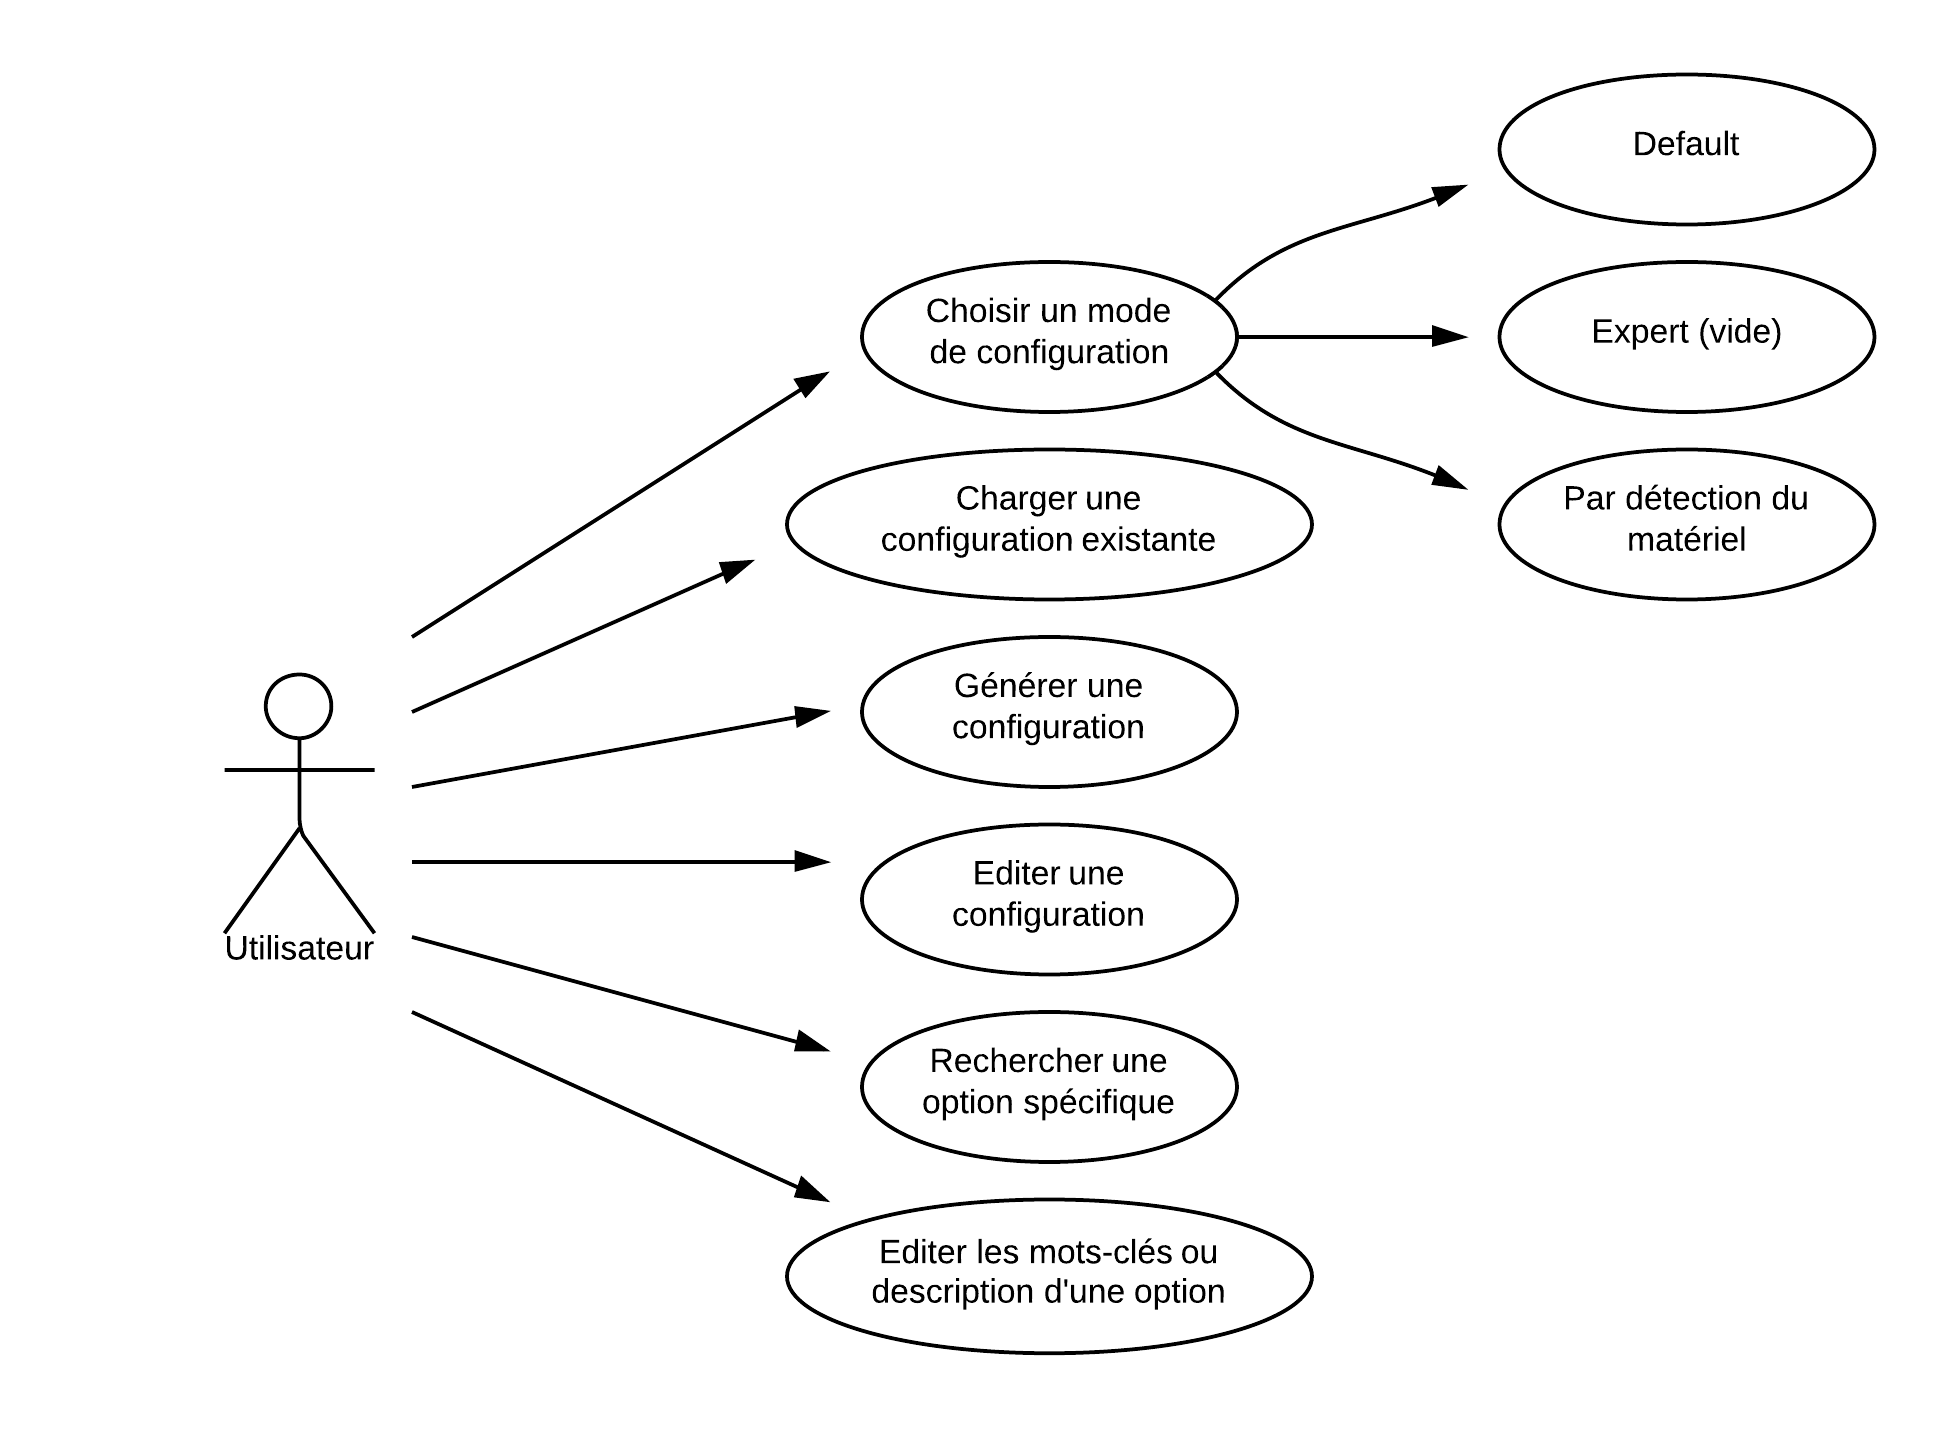
\includegraphics[scale=0.25]{illustrations/diagramme_cas_utilisation.png}


\chapter{Maquettes}
\label{cha:Maquettes}


\section{Écran de démarrage de notre outil}
\label{sec:Écran de démarrage de notre outil}
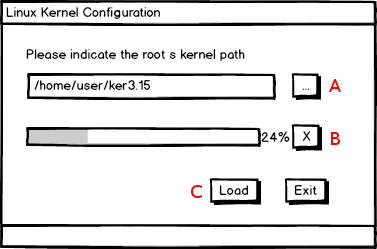
\includegraphics[scale=0.7]{illustrations/first_dialog_an.png} \\

L'utilisateur est invité à fournir le chemin d'un noyau Linux décompressé $[A]$.
L'utilisateur peut charger les options de l'archive en cliquant sur Load $[C]$,
et l'annuler en cliquant sur la X $[B]$ à côté de la barre de chargement.
Il peut quitter l'application à tout moment en cliquant sur Exit.
Lorsque la barre de chargement arrive à 100\%, l'application passe à l'étape
suivante.


\section{Choix d'options de configuration}
\label{sec:Choix d'options de configuration}
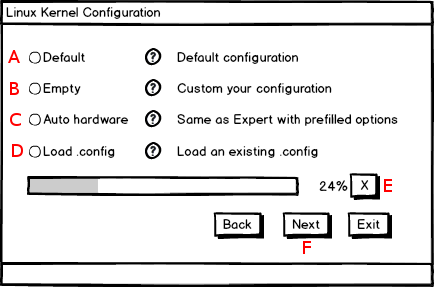
\includegraphics[scale=0.7]{illustrations/choose_dialog_an.png} \\

L'utilisateur pourra retourner à la première étape via le bouton Back.
Il peut quitter l'application à tout moment en cliquant sur Exit.
Pour poursuivre, l'utilisateur devra obligatoirement sélectionner une de ces
quatre options disponibles :

\begin{itemize}
    \item Default $[A]$
    \item Empty $[B]$
    \item Auto hardware $[C]$
    \item Load .config $[D]$
\end{itemize}

Pour chaque possibilité, une description détaillée est disponible en passant le
curseur sur le "?", ainsi qu'un résumé directement visible à droite de ces
éléments d'interface.
Lorsque l'utilisateur veut poursuivre, il clique sur Next $[F]$, ce qui lance
le chargement des options et passe à la fenêtre suivante. Il est possible
d'interrompre le chargement $[E]$ après avoir cliqué sur le bouton Next.


\section{Fenêtre principale de notre outil}
\label{sec:Fenêtre principale de notre outil}
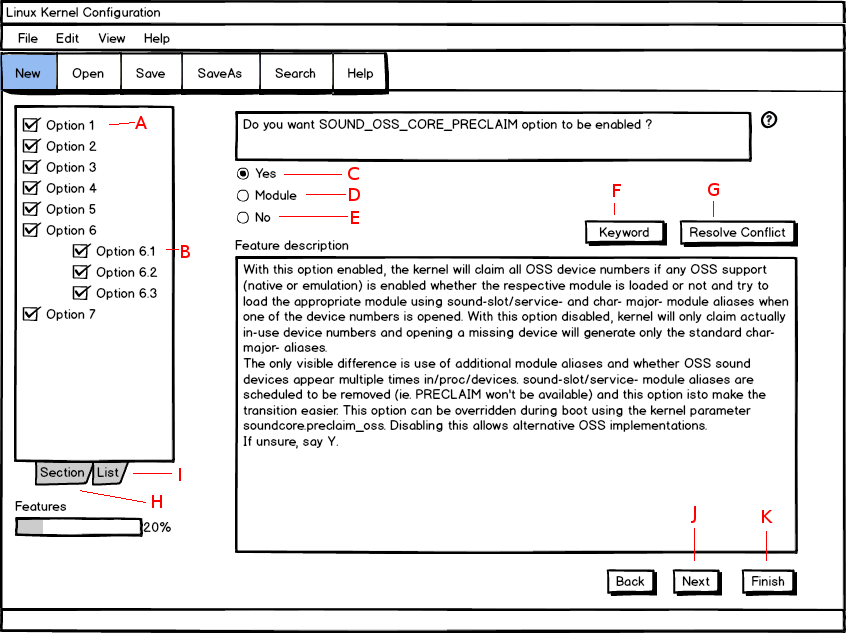
\includegraphics[scale=0.7]{illustrations/MainWindowList_an.png} \\

L'utilisateur est guidé dans sa configuration. Au cours de celle-ci des options
sont proposées, et l'utilisateur peut les accepter dans le noyau $[C]$, en tant
que module $[D]$ ou les désactiver $[E]$. Si un conflit survient, l'utilisateur
ne pourra pas passer à l'étape suivante car le bouton Next $[J]$ sera grisé. Il
faudra qu'il clique sur le bouton $[G]$ qui sera activé afin de résoudre le
conflit. Pour rendre la recherche plus intuitive et pertinente, l'utilisateur
peut rajouter des mots-clés $[F]$ associés à l'option courante.

L'utilisateur pourra changer l'affichage des options en choissisant de les
représenter sous forme de rubriques (maquette ci-dessous) en cliquant sur $[H]$
comme on peut le voir dans l'étude de Waterloo ou on les représentant sous
forme de listes (maquette ci-dessus) en cliquant sur $[I]$ comme dans les
outils existants (xconfig, gconfig).

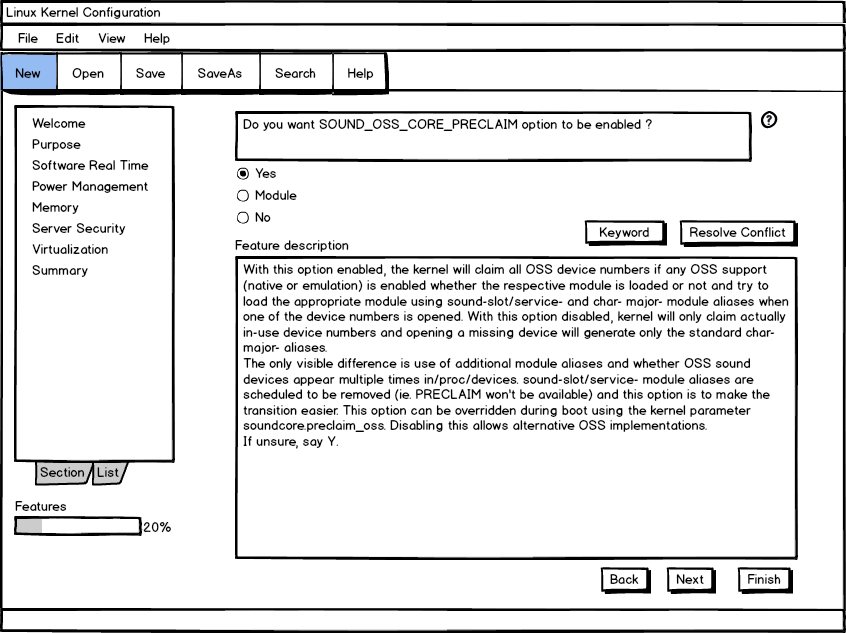
\includegraphics[scale=0.7]{illustrations/MainWindowSection_an.png} \\


\section{Gestion des mots-clés}
\label{sec:Gestion des mots-clés}
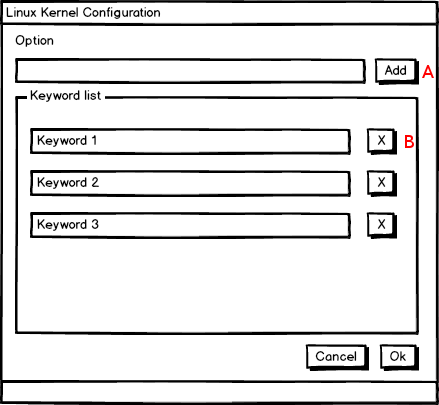
\includegraphics[scale=0.7]{illustrations/keyword_dialog_an.png}

Cette fenêtre s'ouvre lors du choix de configuration à une option donnée quand
est cliqué Keyword sur la fenêtre principale de l'application.
L'utilisateur peut donc voir quels sont les mots-clés associés à cette option,
et peut en ajouter $[A]$ ou supprimer chaque mots-clés existants avec le bouton
X à sa droite $[B]$, s'il le souhaite.


\chapter{Scénarios}
\label{cha:Scénarios}

\section{Scénario A-1 : Configuration par défaut}
\label{sec:Scénario A-1 : Configuration par défaut}

\begin{itemize}
    \item L'utilisateur lance l'application
    \item L'utilisateur sélectionne la configuration par défaut
    \item L'application sélectionne les options génériques pour le
        fonctionnement du noyau Linux voulu
    \item L'utilisateur valide les options présélectionnées par la
        configuration par défaut
    \item L'application génère le fichier .config
    \item L'utilisateur quitte l'application
\end{itemize}


\section{Scénario A-2 : Configuration par défaut, modifications, conflits}
\label{sec:Scénario A-2 : Configuration par défaut, modifications, conflits}

\begin{itemize}
    \item L'utilisateur lance l'application
    \item L'utilisateur sélectionne la configuration par défaut
    \item L'application sélectionne les options génériques pour le
        fonctionnement du noyau Linux voulu
    \item L'utilisateur coche / décoche des options
    \item L'applicaton met en évidence les conflits futurs
    \item L'utilisateur valide les options
    \item L'application génère le fichier .config
    \item L'utilisateur quitte l'application
\end{itemize}


\section{Scénario B : Configuration avancée, modifications, conflits}
\label{sec:Scénario B : Configuration avancée, modifications, conflits}

\begin{itemize}
    \item L'utilisateur lance l'application
    \item L'utilisateur sélectionne la configuration avancée (aucune options
        présélectionnées)
    \item L'utilisateur coche des options
    \item L'application met en évidence les conflits futurs
    \item L'utilisateur essaye de cocher une option qui créerait un conflit
    \item L'application empêche la validation de cette option et affiche un
        bouton de résolution
    \item L'utilisateur clique sur ce bouton et une fenêtre s'ouvre
    \item L'application affiche toutes les options qu'il faudrait décocher pour
        pouvoir résoudre le conflit
    \item L'utilisateur décoche toutes ces options et valide
    \item L'utilisateur valide l'option qui créait des conflits
    \item L'utilisateur valide les options
    \item L'application génère le fichier .config
    \item L'utilisateur quitte l'application
\end{itemize}

\pagebreak

\section{Scénario C : Configuration par détection de matériel et recherche avancée}
\label{sec:Scénario C : Configuration par détection de matériel et recherche avancée}

\begin{itemize}
    \item L'utilisateur lance l'application
    \item L'utilisateur sélectionne la configuration par détection du matériel
    \item L'application sélectionne les options adéquates à la machine actuelle
    \item L'utilisateur coche / décoche des options
    \item L'utilisateur clique sur recherche avancée et saisi un mot-clé pour
        trouver une option
    \item L'application affiche l'option voulue par l'utilisateur
    \item L'utilisateur génère le fichier .config
    \item L'utilisateur quitte l'application
\end{itemize}


\section{Scénario D : Configuration par chargement de fichier de configuration
-- Ajout de mots-clés}
\label{sec:Scénario D : Configuration par chargement de fichier de
configuration -- Ajout de mots-clés}

\begin{itemize}
    \item L'utilisateur lance l'application
    \item L'utilisateur sélectionne le chargement d'une configuration existante
    \item L'application sélectionne les options du fichier
    \item L'utilisateur coche / décoche des options
    \item L'utilisateur se positionne sur une option et clique sur l'ajout de
        mots-clés
    \item L'utilisateur saisit le nom d'un mot-clé et valide l'ajout
    \item L'utilisateur valide les options
    \item L'application génère le fichier .config
    \item L'utilisateur quitte l'application
\end{itemize}


\chapter{Priorité des besoins}
\label{cha:Priorité des besoins}

\begin{tabular}{|c|c|}
    \hline
    Besoin & Priorité \\
    \hline
    \hline
    Génération du fichier .config & Haute \\
    \hline
    Gestion des conflits & Haute \\
    \hline
    Chargement d'un fichier .config & Haute \\
    \hline
    Utilisation de l'application sur un bureau & Haute \\
    \hline
    Recherche & Haute \\
    \hline
    Mots-clés et description d'une option & Moyenne \\
    \hline
    Plateforme de partage commnunautaire & Moyenne \\
    \hline
    Détection du matériel & Moyenne \\
    \hline
    Peuplement de la base pour la détection de matériel & Faible \\
    \hline
    Utilisation de l'application sur un serveur & Faible \\
    \hline
\end{tabular}


\chapter{Tests}
\label{cha:Tests}

\section{Validité du fichier de configuration}
\label{sec:Validité du fichier de configuration}

Vérifier que le fichier de configuration (.config) soit compatible avec
l'application lors de son chargement. Ce dernier doit respecter le format
d'origine, afin que nous puissions récupérer les informations qui nous sont
utiles.

Vérifier que le fichier de configuration que nous générons via notre outil
puisse être chargé (toujours avec notre outil) et qu'il contienne les mêmes
données. Pour réaliser ce test, on générera à nouveau un fichier de
configuration et on pourra vérifier après ces trois étapes (génération >
chargement > génération) si les informations sont restées les mêmes. Cela
montrera que la génération et le chargement fonctionnent correctement.


\section{Gestion des conflits}
\label{sec:Gestion des conflits}

La sélection d'une option doit signaler à l'utilisateur l'eventuelle présence
d'un conflit. Il doit également lui être proposé de pouvoir le résoudre. Or,
trouver une solution est un problème NP-complet. En effet, à chaque nouvelle
option il faut vérifier les dépendances de toutes les options précédemment
cochées. Il est possible qu'une option précédente exclût la nouvelle option.
Toutes les options du fichier de configuration en cours d'édition doivent être
vérifiées, ce qui est impossible en un temps polynomial.

Il faudrait vérifier que les conflits présents dans les fichiers Kconfig du
noyau soient bien affichés dans notre outil.


\section{Système de recherche}
\label{sec:Système de recherche}

Vérifier que la fonction de recherche retourne bien les résultats attendus.
Par exemple, nous pourrons oubrir un des outils existants (xconfig, gconfig) et
réaliser une recherche. On effectuera la même recherche sur notre outil et on
pourra vérifier si les résultats sont similaires (ce test ne sera valable que
pour les titres des options).


\section{Compatibilité}
\label{sec:Compatibilité}

Si l'utilisateur précise qu'il réalise une configuration pour la machine
courante, l'application decra l'alerter quand celui-ci cherchera à activer une
option incompatible avec son matériel. Par exemple, si sa machine a un
processeur 32-bits et que l'utilisateur sélectionne l'option pour un processeur
64-bits, l'application devra l'avertir que la configuration ne sera pas adaptée
à sa machine.


\section{Interface graphique}
\label{sec:Interface graphique}

Nous allons vérifier la fiabilité de l'interface graphique. Chaque interfaction
possible avec les éléments de l'interface doit réaliser l'action attendue.


\end{document}
